% MODIFICA EL CONTENIDO QUE VIENE A CONTINUACIÓN DE ACUERDO A TU TRABAJO

\chapter{Problema del Bandido de $k$-brazos}

%%%%%%%%%%%%%%%%%%%%%%%%%%%%%%%%%%%%%%%%%%%%%%%%%%%%%%%%%%%%%
%%%%%%%%%%%%%%%%%%%%%%%%%%%%%%%%%%%%%%%%%%%%%%%%%%%%%%%%%%%%%
\section{Introducción}

\subsection{Descripción del problema y relevancia}
El problema del \textbf{Bandido Multibrazo} (o \textit{k-armed bandit}) modela una situación clásica 
de toma de decisiones secuencial bajo incertidumbre en entornos estacionarios. En este escenario, 
un agente se enfrenta a una máquina con $k$ palancas o "brazos", donde cada uno ofrece una recompensa 
que sigue una distribución de probabilidad desconocida para el agente. 
De esta manera, el objetivo es maximizar la recompensa acumulada a lo largo de un horizonte temporal $T$.

La relevancia de este problema radica en que se trata de un caso fundamental en el campo del Aprendizaje por Refuerzo, 
sirviendo como ejemplo básico del \textbf{dilema de la Exploración-Explotación}.
El agente debe decidir continuamente entre explotar el brazo que cree que ofrece 
la mayor recompensa (basándose en su conocimiento actual) o explorar otros brazos 
para recabar más información, arriesgándose a obtener recompensas menores a corto plazo pero 
con la posibilidad de descubrir opciones óptimas a largo plazo.

\subsection{Motivación del trabajo}
El estudio del bandido de $k$-brazos es crucial no solo como base teórica para comprender 
problemas más complejos, sino por su aplicabilidad directa en problemas del mundo real.

Ejemplos tangibles de estas aplicaciones incluyen 
la \textbf{optimización de campañas de publicidad online} (donde se modela la tasa de clics 
o CTR mediante distribuciones de Bernoulli), la \textbf{personalización de recomendaciones} 
en plataformas de streaming , o la \textbf{asignación de promociones} en aplicaciones de \textit{delivery}.

La motivación principal de este trabajo es comprender cómo diferentes estrategias algorítmicas y 
distribuciones de recompensa afectan al rendimiento de los agentes en este entorno.



\subsection{Objetivos del informe}
El objetivo principal de este informe técnico es realizar un estudio comparativo riguroso de 
diferentes familias de algoritmos de aprendizaje por refuerzo aplicados al 
problema del bandido de $k$-brazos. Los objetivos específicos son:

\begin{itemize}
    \item \textbf{Implementación de Algoritmos:} Desarrollar y validar algoritmos representativos 
    de las familias $\epsilon$-Greedy, Softmax y UCB1/UCB2.
    \item \textbf{Análisis Experimental:} Evaluar el rendimiento de dichos algoritmos en entornos 
    con distintas distribuciones de recompensa (Normal, Bernoulli y Binomial), siempre 
    considerando las mismas recompensas de cada brazo para garantizar una comparación justa.
    \item \textbf{Evaluación de Métricas:} Analizar la eficacia de los agentes mediante las métricas de 
    Recompensa Promedio, Porcentaje de Selección del Brazo Óptimo, Estadísticas por Brazo y Regret Acumulado.
    \item \textbf{Estudio de Hiperparámetros:} Investigar cómo afectan parámetros como la tasa 
    de exploración $\epsilon$ o la temperatura $\tau$ en el comportamiento de convergencia y estabilidad 
    de los agentes.
\end{itemize}

\subsection{Organización del documento}
El resto del presente documento se estructura de la siguiente manera:

\begin{itemize}
    \item En la \textbf{Sección 2}, se detallan los fundamentos teóricos de los algoritmos 
    implementados ($\epsilon$-Greedy, Softmax, UCB1), así como antecedentes relevantes en la literatura 
    sobre el problema en cuestión.
    \item La \textbf{Sección 3} describe la metodología experimental, incluyendo la explicación 
    de los algoritmos implementados.
    \item La \textbf{Sección 4} presenta los resultados experimentales obtenidos, para lo cual 
    se incluyen gráficos y métricas, junto con un análisis crítico de los mismos. También se realizan comparaciones
    en el caso de $\epsilon$-Greedy con $\epsilon$-decaimiento y UCB1 con UCB2.
    \item Finalmente, en la \textbf{Sección 5}, se exponen las conclusiones principales derivadas del estudio.
\end{itemize}

\section{Desarrollo}

En esta sección se formaliza el problema abordado, se revisa el estado del arte y se 
detallan los métodos algorítmicos implementados para la resolución del dilema de exploración-explotación.

\subsection{Definición Formal del Problema}
El problema del Bandido de $k$-brazos se modela como un proceso de decisión 
secuencial de un solo estado. Formalmente, definimos un conjunto de acciones 
$\mathcal{A} = \{1, \dots, k\}$, donde cada acción $a$ corresponde a la selección de uno de los brazos de la máquina.

En cada paso de tiempo discreto $t = 1, 2, \dots, T$, el agente selecciona una acción $A_t \in \mathcal{A}$ y 
recibe una recompensa numérica $R_t$. Esta recompensa proviene de una distribución de probabilidad 
asociada al brazo seleccionado, $\mathcal{P}_a$, tal que $R_t \sim \mathcal{P}_{A_t}$. 
El valor esperado de la recompensa para una acción $a$ se denota como:
\begin{equation}
    q(a) = \mathbb{E}[R_t | A_t = a] 
\end{equation}

El objetivo del agente es maximizar la recompensa total acumulada a lo largo del horizonte temporal $T$.

\subsection{Enfoques Existentes y Estado del Arte}
La literatura del aprendizaje por refuerzo clasifica las estrategias de resolución del problema del bandido en función de cómo gestionan la incertidumbre de las estimaciones $Q_t(a) \approx q_*(a)$.

Los enfoques clásicos se dividen en:
\begin{itemize}
    \item \textbf{Métodos Voraces (Greedy) y $\epsilon$-Greedy:} Son los enfoques más simples, donde el agente alterna entre explotar el conocimiento actual con probabilidad $1-\epsilon$ y explorar aleatoriamente con probabilidad $\epsilon$. Aunque efectivos, no consideran la varianza de las estimaciones.
    \item \textbf{Métodos de Intervalo de Confianza (UCB):} Basados en el principio de ``optimismo ante la incertidumbre'', estos algoritmos (como UCB1) seleccionan acciones basándose en el límite superior de un intervalo de confianza, favoreciendo acciones poco exploradas de manera determinista.
    \item \textbf{Métodos de Gradiente y Softmax:} A diferencia de los anteriores, que estiman valores de acción, 
    estos métodos aprenden una preferencia numérica $H_t(a)$ para cada acción o 
    utilizan una distribución de probabilidad de Boltzmann (Softmax) dependiente de 
    una temperatura $\tau$, permitiendo una selección de cada acción proporcional a su preferencia relativa.
\end{itemize}

\subsection{Contexto y Aplicaciones Específicas}
Aunque el problema se define teóricamente con distribuciones genéricas, este trabajo aborda su aplicación en contextos específicos modelados mediante distintas distribuciones de probabilidad, las cuales representan escenarios reales de toma de decisiones:
\begin{itemize}
    \item \textbf{Distribución de Bernoulli:} Modela escenarios de éxito/fracaso binario, como la tasa de clics (CTR) en publicidad online ($R_t \in \{0, 1\}$).
    \item \textbf{Distribución Binomial:} Representa situaciones donde una acción se aplica a un lote de $n$ usuarios, obteniendo un número de éxitos $k$ (e.g., optimización de promociones en apps de \textit{delivery}).
    \item \textbf{Distribución Normal:} Utilizada cuando la recompensa es una variable continua, adecuada para métricas de interacción de usuario como el tiempo de visualización en plataformas de \textit{streaming}.
\end{itemize}

\subsection{Métodos Utilizados}
Para abordar el problema planteado, se han implementado y comparado tres familias de algoritmos, cada una con un mecanismo distinto de gestión del compromiso exploración-explotación.

\subsubsection{Algoritmo $\epsilon$-Greedy}
Este método mantiene estimaciones $Q_t(a)$ del valor de cada brazo mediante promedios muestrales. La regla de selección de acción es:
\begin{equation}
    A_t = \begin{cases}
    \operatorname{argmax}_a Q_t(a) & \text{con probabilidad } 1 - \epsilon \\
    \text{acción aleatoria} & \text{con probabilidad } \epsilon
    \end{cases}
\end{equation}
Se han realizado experimentos variando $\epsilon$ para analizar su impacto en la convergencia.



\subsubsection{Algoritmo $\epsilon$-decaimiento}
Como variante del anterior, se ha implementado una versión de $\epsilon$-Greedy con decaimiento inversamente proporcional al tiempo, lo que permite una exploración más intensa en las etapas iniciales y una mayor explotación a medida que se acumula información:
\begin{equation}
    \epsilon_t = \max\left(\epsilon_{min}, \frac{\epsilon_0}{1 + \lambda_{decay} t}\right)
\end{equation}
donde $\epsilon_0$ es el valor inicial de exploración, $\lambda_{decay}$ controla la velocidad de decaimiento y $\epsilon_{min}$ garantiza un nivel mínimo de exploración a largo plazo.


\subsubsection{Algoritmo Softmax (Distribución de Gibbs)}
Este método selecciona acciones basándose en probabilidades calculadas mediante una distribución de Boltzmann. La probabilidad de seleccionar la acción $a$ en el tiempo $t$ viene dada por:
\begin{equation}
    \pi_t(a) = \frac{e^{Q_t(a)/\tau}}{\sum_{b=1}^{k} e^{Q_t(b)/\tau}}
\end{equation}
donde el parámetro de temperatura $\tau$ regula la aleatoriedad de la selección. Valores altos de $\tau$ tienden a la equiprobabilidad (exploración pura), mientras que $\tau \to 0$ tiende a una política voraz (explotación pura).

\subsubsection{Algoritmo UCB1 (Upper Confidence Bound)}
El algoritmo UCB1 evita la aleatoriedad explícita y selecciona acciones maximizando una cota superior de confianza:
\begin{equation}
    A_t = \operatorname{argmax}_a \left[ Q_t(a) + c \sqrt{\frac{\ln t}{N_t(a)}} \right]
\end{equation}
donde $N_t(a)$ es el número de veces que la acción $a$ ha sido seleccionada y $c$ es una constante que controla el grado de exploración. Este término adicional fuerza la exploración de brazos poco visitados a medida que $t$ aumenta.

\subsubsection{Algoritmo UCB2}
Como extensión del anterior, se ha implementado el algoritmo UCB2, el cual introduce una estructura de \textbf{épocas} para mejorar la eficiencia de la exploración. A diferencia de UCB1, que reevalúa la decisión en cada paso $t$, UCB2 selecciona un brazo y lo mantiene activo durante un intervalo de tiempo determinado por una función de crecimiento geométrico:
\begin{equation}
    \tau(r) = \lceil (1+\alpha)^r \rceil
\end{equation}
donde $\alpha > 0$ es un parámetro que regula el incremento de las épocas. Esta estrategia reduce la frecuencia de cambio entre brazos y permite obtener teóricamente mejores cotas de rechazo asintótico al amortizar el coste de exploración en intervalos más largos.

%%%%%%%%%%%%%%%%%%%%%%%%%%%%%%%%%%%%%%%%%%%%%%%%%%%%%%%%%%%%%
%%%%%%%%%%%%%%%%%%%%%%%%%%%%%%%%%%%%%%%%%%%%%%%%%%%%%%%%%%%%%
\section{Algoritmos}

En este capítulo se detallan los procedimientos algorítmicos seleccionados para abordar el problema del bandido de $k$-brazos. Se han elegido tres estrategias representativas de las familias más importantes de aprendizaje por refuerzo en este contexto: métodos voraces con exploración aleatoria ($\epsilon$-Greedy), métodos probabilísticos basados en gradiente de valor (Softmax) y métodos de intervalo de confianza determinista (UCB1).

\subsection{Algoritmo $\epsilon$-Greedy}

\subsubsection{Descripción y Justificación}
El algoritmo $\epsilon$-Greedy es la estrategia base por excelencia en el aprendizaje por refuerzo. Su elección se justifica por su simplicidad y su capacidad para establecer una línea base (\textit{baseline}) de rendimiento. Funciona alternando entre dos comportamientos controlados por el hiperparámetro $\epsilon \in [0, 1]$:
\begin{itemize}
    \item \textbf{Explotación:} Con probabilidad $1-\epsilon$, selecciona el brazo con el mayor valor estimado $Q_t(a)$ hasta el momento.
    \item \textbf{Exploración:} Con probabilidad $\epsilon$, selecciona un brazo de forma uniformemente aleatoria, garantizando que todas las acciones tengan una probabilidad no nula de ser elegidas a largo plazo.
\end{itemize}

\subsubsection{Pseudocódigo}
\begin{algorithm}
\caption{Algoritmo $\epsilon$-Greedy}
\begin{algorithmic}[1] 
\Require $k$ (número de brazos), $\epsilon$ (probabilidad), $T$ (horizonte)
\State Inicializar $Q(a) \gets 0$ y $N(a) \gets 0$ para todo $a \in \{1, \dots, k\}$
\For{$t \gets 1$ \textbf{to} $T$}
    \State Generar número aleatorio $\xi \in [0, 1]$
    \If{$\xi < \epsilon$}
        \State Seleccionar brazo $A_t$ aleatoriamente de $\{1, \dots, k\}$
    \Else
        \State Seleccionar $A_t = \operatorname{argmax}_a Q(a)$
    \EndIf
    \State Recibir recompensa $R_t$ del brazo $A_t$
    \State $N(A_t) \gets N(A_t) + 1$
    \State $Q(A_t) \gets Q(A_t) + \frac{1}{N(A_t)} (R_t - Q(A_t))$
\EndFor
\end{algorithmic}
\end{algorithm}

\subsection{Algoritmo Softmax (Distribución de Gibbs)}

\subsubsection{Descripción y Justificación}
A diferencia de $\epsilon$-Greedy, el algoritmo Softmax asigna probabilidades de selección 
proporcionales al valor estimado de cada brazo. Se justifica su inclusión porque representa 
una estrategia más sofisticada que penaliza las acciones con un rendimiento más pobre, concentrando 
la exploración en las acciones que son casi tan buenas como la óptima, evitando así probar 
iteradamente las peores opciones, como sí hace $epsilon$-greedy. La temperatura $\tau$ regula la sensibilidad de estas 
probabilidades ante las diferencias en los valores $Q$.

\subsubsection{Pseudocódigo}
\begin{algorithm}
\caption{Algoritmo Softmax}
\begin{algorithmic}[1]
\Require $k$, $\tau$ (temperatura), $T$ (horizonte)
\State Inicializar $Q(a) \gets 0$ y $N(a) \gets 0$ para todo $a$
\For{$t \gets 1$ \textbf{to} $T$}
    \State Calcular denominador $S \gets \sum_{b=1}^{k} e^{Q(b)/\tau}$
    \For{$a \gets 1$ \textbf{to} $k$}
        \State $\pi_t(a) \gets \frac{e^{Q(a)/\tau}}{S}$
    \EndFor
    \State Seleccionar brazo $A_t$ muestreando de la distribución $\pi_t$
    \State Recibir recompensa $R_t$
    \State $N(A_t) \gets N(A_t) + 1$
    \State $Q(A_t) \gets Q(A_t) + \frac{1}{N(A_t)} (R_t - Q(A_t))$
\EndFor
\end{algorithmic}
\end{algorithm}

\subsection{Algoritmo UCB1 (Upper Confidence Bound)}

\subsubsection{Descripción y Justificación}
El algoritmo UCB1 se no utiliza aleatoriedad, sino que selecciona acciones maximizando una cota superior 
del intervalo de confianza. 

La inclusión del algoritmo UCB1 y su variante UCB2 en este estudio comparativo  se justifica por dos factores críticos:

\begin{itemize}
    \item \textbf{Garantías de Convergencia:} Auer et al. (2002) \cite{auer2002}  demostraron que UCB1 garantiza una cota 
    de rechazo acumulado (\textit{regret}) que crece de manera logarítmica con respecto al tiempo ($O(\ln T)$). 
    Esto asegura que el número de selecciones subóptimas se minimiza asintóticamente de forma eficiente.
    
    \item \textbf{Adaptabilidad Automática:} El algoritmo gestiona el compromiso exploración-explotación sin 
    requerir la disminución manual de parámetros (como es el caso del decaimiento de $\epsilon$ o $\tau$ en Softmax). 
    El término de exploración $\sqrt{\frac{\ln t}{N_t(a)}}$ crece con el tiempo global ($t$) 
    pero decrece con las visitas locales ($N_t(a)$), forzando al sistema a explorar brazos poco 
    visitados inicialmente y a converger naturalmente hacia la explotación del brazo óptimo conforme se reduce la incertidumbre.
\end{itemize}

\subsubsection{Pseudocódigo}
\begin{algorithm}
\caption{Algoritmo UCB1}
\begin{algorithmic}[1]
\Require $k$, $T$ (horizonte)
\State \Comment{Inicialización: probar cada brazo una vez}
\For{$a \gets 1$ \textbf{to} $k$}
    \State Seleccionar brazo $a$
    \State Recibir recompensa $R$, actualizar $Q(a)$, $N(a) \gets 1$
\EndFor
\State \Comment{Bucle principal}
\For{$t \gets k+1$ \textbf{to} $T$}
    \State Seleccionar brazo $A_t$ que maximice:
    \State \quad $A_t = \operatorname{argmax}_a \left( Q(a) + \sqrt{\frac{2 \ln t}{N(a)}} \right)$
    \State Recibir recompensa $R_t$
    \State $N(A_t) \gets N(A_t) + 1$
    \State $Q(A_t) \gets Q(A_t) + \frac{1}{N(A_t)} (R_t - Q(A_t))$
\EndFor
\end{algorithmic}
\end{algorithm}
%%%%%%%%%%%%%%%%%%%%%%%%%%%%%%%%%%%%%%%%%%%%%%%%%%%%%%%%%%%%%
%%%%%%%%%%%%%%%%%%%%%%%%%%%%%%%%%%%%%%%%%%%%%%%%%%%%%%%%%%%%%
\section{Evaluación y Experimentos}

En este capítulo se detallan las pruebas realizadas para evaluar el desempeño de los algoritmos implementados. El objetivo es analizar cómo se comportan las distintas estrategias de exploración-explotación bajo diferentes distribuciones de recompensa y configuraciones de hiperparámetros.

\subsection{Configuración Experimental}

\subsubsection{Entornos de Prueba}
Se han utilizado tres tipos de entornos de prueba basados en diferentes distribuciones de 
recompensa:
\begin{itemize}
    \item \textbf{Distribución Normal ($\mathcal{N}(\mu, \sigma^2)$):} Simula recompensas continuas. Se configuraron $k=10$ brazos con medias $\mu \in [1, 10]$ y desviación estándar $\sigma=1$.
    \item \textbf{Distribución de Bernoulli ($\mathcal{B}(p)$):} Simula recompensas binarias (éxito/fracaso). Se utilizaron $k=10$ brazos con probabilidades de éxito $p \in [0.1, 1.0]$.
    \item \textbf{Distribución Binomial ($\mathcal{B}(n, p)$):} Simula recompensas discretas agregadas (número de éxitos en $n$ intentos). Se configuraron $k=10$ brazos con $n=10$ y $p \in [0.1, 1.0]$.
\end{itemize}

\subsubsection{Herramientas y Reproducibilidad}
Los experimentos se han implementado en Python utilizando \textit{notebooks} de Jupyter alojados en Google Colab. 
Para asegurar la reproducibilidad de los experimentos, se ha fijado una semilla aleatoria (\texttt{seed}) 
constante en todas las ejecuciones y se han utilizado las mismas recompensas para cada brazo en todas las estrategias comparadas,
garantizando así una comparación justa y directa entre los algoritmos.

\subsubsection{Métricas de Desempeño}
Para cuantificar la calidad de las estrategias, se han monitorizado las siguientes métricas a lo largo 
de un horizonte temporal de $T=1000$ pasos (a excepción de la familia Softmax en la que se han utilizado 3000 pasos
ya que presentaba una convergencia más lenta), promediando los resultados sobre 500 ejecuciones independientes ($runs$):
\begin{enumerate}
    \item \textbf{Recompensa Promedio:} Evolución del valor medio obtenido en cada paso de tiempo.
    \item \textbf{Porcentaje de Selección Óptima:} Proporción de veces que el agente selecciona el brazo con la mayor esperanza matemática ($\mu^*$).
    \item \textbf{Rechazo Acumulado (\textit{Regret}):} La diferencia acumulada entre la recompensa óptima esperada y la obtenida por el agente.
    \item \textbf{Estadísticas por Brazo:} Histograma de selecciones que permite visualizar si el agente convergió al brazo óptimo o quedó atrapado en óptimos locales.
\end{enumerate}


\subsection{Resultados: Familia $\epsilon$-Greedy}

Se evaluó el algoritmo $\epsilon$-Greedy para valores $\epsilon \in \{0, 0.01, 0.1\}$, así como su variante con decaimiento ($\epsilon$-decaimiento). A diferencia de Softmax, esta familia incluye una fase de exploración inicial explícita.

Para todas las distribuciones se observó que:

\begin{itemize}
    \item \textbf{$\epsilon = 0$ (Explotación pura):} Tras la exploración inicial forzada, el agente selecciona siempre el brazo con mayor recompensa estimada. 
    En el experimento base con distribución Normal ($\sigma = 1$), este enfoque obtuvo un rendimiento muy alto, ya que en la mayoría de las ejecuciones la estimación inicial fue suficientemente representativa como para identificar correctamente el brazo óptimo desde el principio. 
    No obstante, su comportamiento es extremadamente sensible al ruido: cuando la estimación inicial es errónea, el algoritmo queda atrapado en un brazo subóptimo durante toda la ejecución. Hechos que quedaron evidenciados al aumentar la desviación típica a $\sigma = 10$, donde el rendimiento se desplomó debido a la alta probabilidad de obtener muestras iniciales no representativas.

    \item \textbf{$\epsilon = 0.01$ (Exploración baja):} Introduce una exploración moderada (1\% de las veces), lo que permite corregir posibles errores iniciales sin penalizar excesivamente la explotación. 
    Su convergencia es más lenta que la de $\epsilon=0.1$ en las primeras etapas, pero a largo plazo alcanza recompensas promedio muy cercanas al óptimo, ya que la probabilidad de seleccionar brazos subóptimos es muy reducida.

    \item \textbf{$\epsilon = 0.1$ (Exploración alta):} Aprende con mayor rapidez durante las primeras iteraciones, ya que explora con mayor frecuencia y detecta antes el brazo óptimo. 
    Sin embargo, su recompensa promedio se estabiliza por debajo del óptimo teórico, debido a que mantiene permanentemente una probabilidad del 10\% de seleccionar brazos subóptimos.

    \item \textbf{$\epsilon$-decaimiento:} Comienza con una exploración elevada ($\epsilon_0 = 1.0$) y la reduce progresivamente según la función 
    $$
    \epsilon(t) = \frac{\epsilon_0}{1 + \lambda t},
    $$
    con un mínimo $\epsilon_{min}=0.01$. 
    Este esquema combina una exploración intensiva inicial con una explotación dominante a largo plazo, logrando el mejor compromiso global entre rapidez de aprendizaje y rendimiento final.
\end{itemize}

La Figura~\ref{fig:egreedy_reward_normal} muestra la evolución de la recompensa promedio en el caso base con distribución Normal ($\sigma=1$).

\begin{figure}[H]
    \centering
    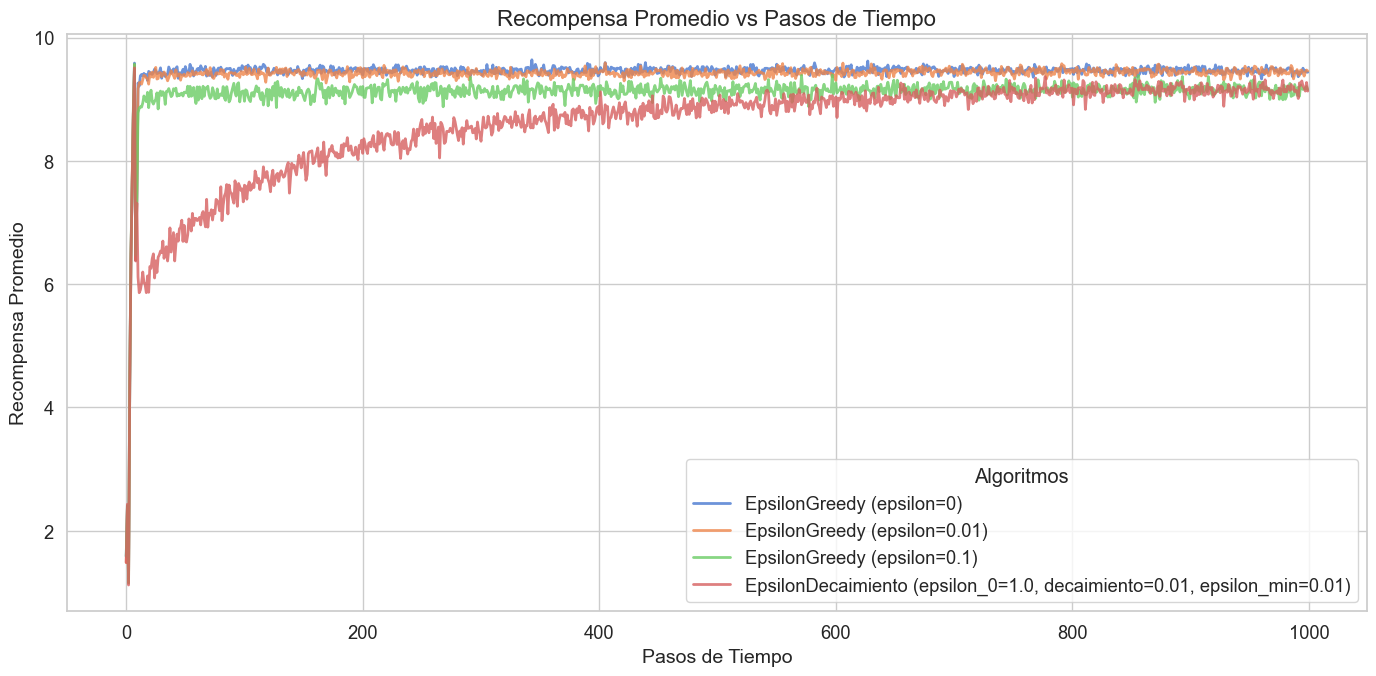
\includegraphics[width=0.5\textwidth]{resources/egreedy_reward_normal_sigma1.png}
    \caption{Recompensa promedio en función del número de pasos para la familia $\epsilon$-Greedy bajo distribución Normal con $\sigma=1$.}
    \label{fig:egreedy_reward_normal}
\end{figure}

% En términos de \textbf{regret acumulado}, todos los algoritmos presentan inicialmente un crecimiento rápido debido a la fase de exploración. Sin embargo:

% \begin{itemize}
%     \item Para $\epsilon=0$, el regret se estabiliza rápidamente si la estimación inicial fue correcta, pero puede crecer linealmente en las ejecuciones donde el algoritmo se estanca en un brazo subóptimo.
%     \item Para $\epsilon>0$, el regret crece de manera aproximadamente lineal a largo plazo, debido a la exploración constante.
%     \item El algoritmo $\epsilon$-decaimiento presenta el crecimiento más controlado, ya que la exploración disminuye con el tiempo, reduciendo progresivamente la contribución al regret.
% \end{itemize}

\paragraph{Impacto de la varianza en la distribución Normal.}

Al aumentar la desviación típica a $\sigma = 10$, se observó una degradación significativa en el rendimiento de $\epsilon=0$. 
La elevada varianza hace que las muestras iniciales sean poco representativas de la media real de cada brazo, incrementando la probabilidad de seleccionar incorrectamente un brazo subóptimo y explotarlo durante toda la ejecución.

En contraste, los algoritmos con exploración ($\epsilon=0.01$, $\epsilon=0.1$ y $\epsilon$-decaimiento) logran corregir estas estimaciones erróneas gracias a la exploración continua, superando claramente al caso puramente explotador.

Por el contrario, al reducir la desviación típica a $\sigma = 0.1$, las muestras iniciales se vuelven altamente representativas. En este escenario, $\epsilon=0$ alcanza el 100\% de selección del brazo óptimo en todas las ejecuciones, convirtiéndose en la mejor estrategia.

Este efecto puede observarse claramente en la Figura~\ref{fig:egreedy_variance_effect}, donde se observa cómo afecta al porcentaje de selección del brazo óptimo el hecho de que la desviación típica sea $\sigma=10$.

\begin{figure}[H]
    \centering
    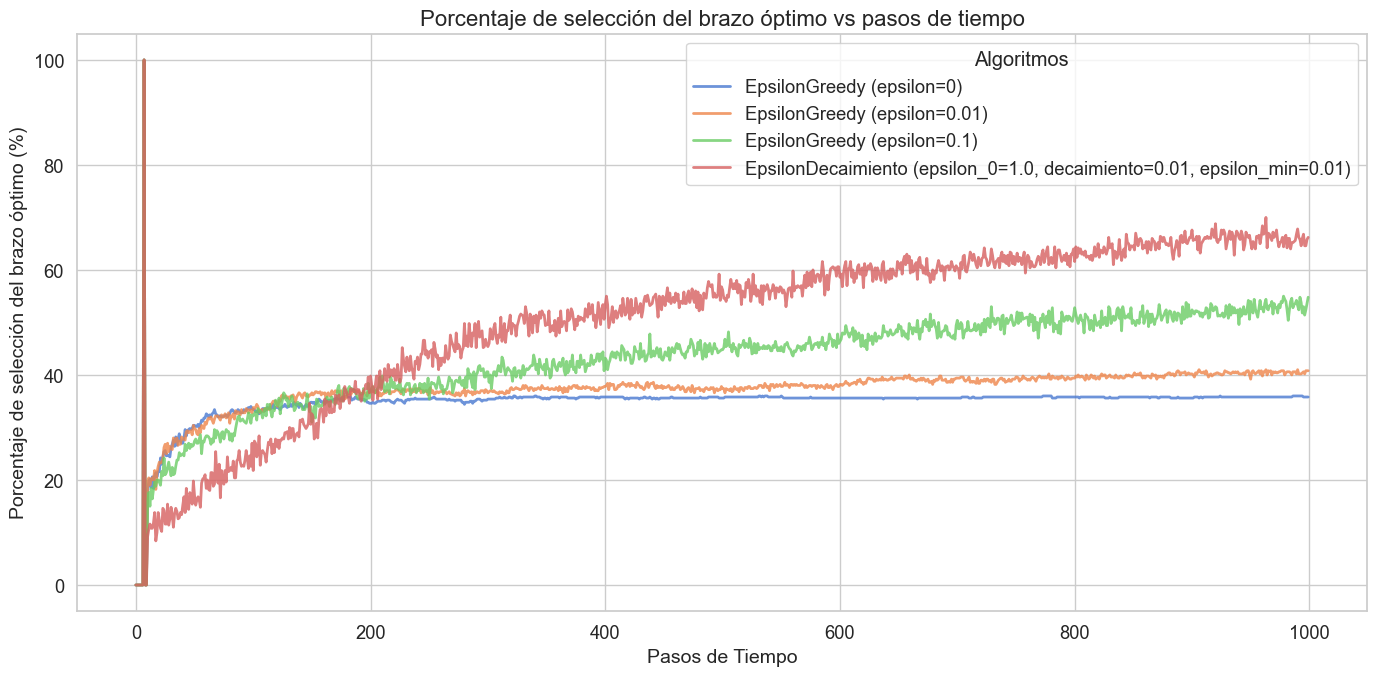
\includegraphics[width=0.5\textwidth]{resources/egreedy_variance_comparison.png}
    \caption{Porcentaje de selección del brazo óptimo para $\sigma=10$ en la familia $\epsilon$-Greedy.}
    \label{fig:egreedy_variance_effect}
\end{figure}

\paragraph{Resultados en la distribución de Bernoulli.}

En la distribución de Bernoulli (recompensas 0 o 10), el ruido discreto introduce numerosos empates en las estimaciones iniciales y una elevada varianza en las primeras fases. Esto afecta especialmente a $\epsilon=0$ y $\epsilon=0.01$, que pueden quedar temporalmente atrapados en brazos subóptimos si el brazo óptimo falla en las primeras muestras, como se puede observar en la Figura~\ref{fig:egreedy_discrete}.

No obstante, conforme aumenta el número de observaciones, las medias estimadas se estabilizan y todos los algoritmos mejoran progresivamente su porcentaje de selección del brazo óptimo.

En este entorno, el algoritmo $\epsilon$-decaimiento mostró el comportamiento más robusto, ya que su fuerte exploración inicial le permite identificar correctamente el brazo óptimo incluso cuando las primeras observaciones son desfavorables.

\begin{figure}[H]
    \centering
    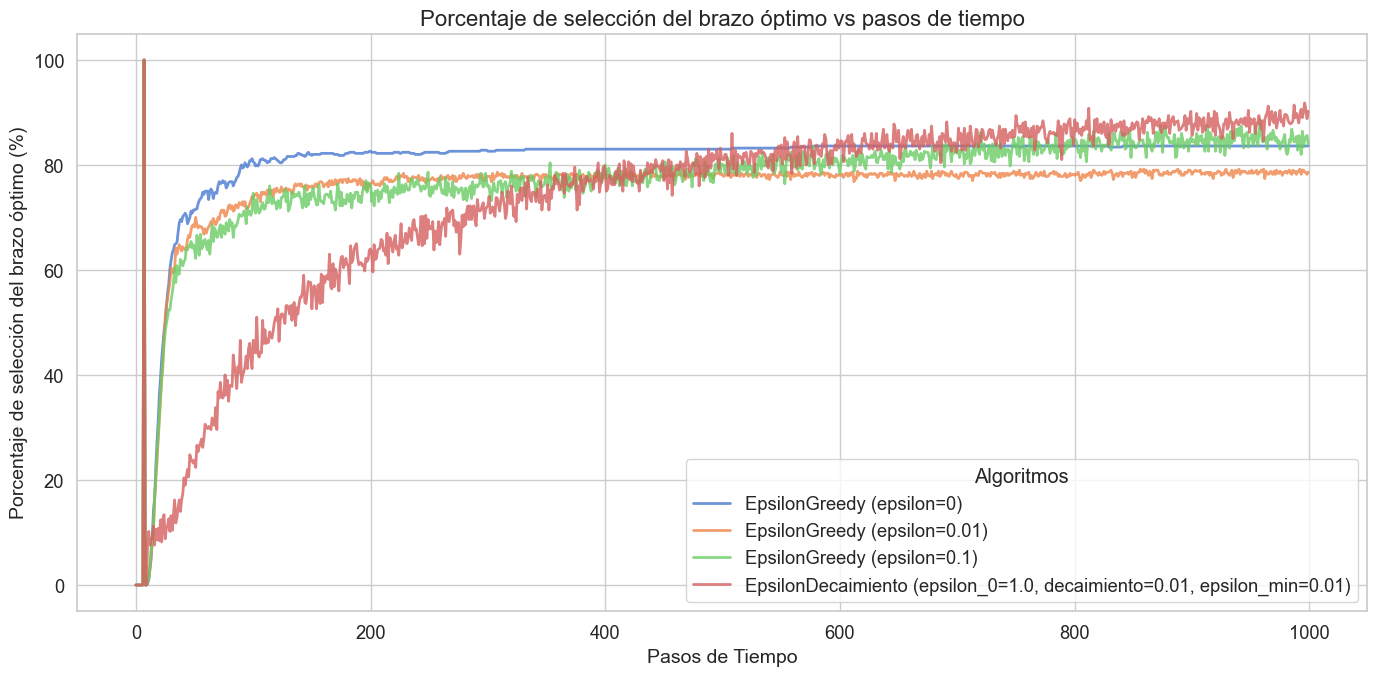
\includegraphics[width=0.5\textwidth]{resources/egreedy_bernoulli_binomial.png}
    \caption{Porcentaje de selección del brazo óptimo en distribuciones Bernoulli para los algoritmos $\epsilon$-Greedy.}
    \label{fig:egreedy_discrete}
\end{figure}

\paragraph{Resultados en la distribución Binomial.}

En la distribución Binomial ($n=10$), la varianza es menor que en la Bernoulli pura, ya que cada recompensa es la suma de varios ensayos independientes. Esto reduce los empates y estabiliza las estimaciones más rápidamente.

Como consecuencia, el comportamiento observado es muy similar al caso Normal: todos los algoritmos logran identificar el brazo óptimo con el tiempo, siendo $\epsilon$-decaimiento y $\epsilon=0.01$ los que presentan el mejor rendimiento global a largo plazo.

En conjunto, los resultados muestran que el desempeño de la familia $\epsilon$-Greedy depende críticamente del equilibrio entre exploración y explotación y de la varianza de la distribución de recompensas. 
Una exploración constante elevada acelera el aprendizaje inicial pero penaliza el rendimiento final, mientras que la ausencia total de exploración solo es adecuada cuando las estimaciones iniciales son fiables. 
La estrategia con decaimiento emerge como la opción más robusta y eficiente en entornos con incertidumbre moderada o alta.




\subsection{Resultados: Familia Softmax}
Se evaluó el algoritmo Softmax variando la temperatura $\tau \in \{0.1, 1.0, 5.0\}$.

Para todas las distribuciones, se observó que:
\begin{itemize}
    \item \textbf{Temperatura Baja ($\tau=0.1$):} El agente se comportó de manera casi voraz, explotando rápidamente el primer 
    brazo que visitó. Esto se debe a que Softmax no incluye una primera pasada de exploración forzada, 
    lo que hace que la primera acción seleccionada tenga un impacto desproporcionado en las estimaciones iniciales. 
    Esto provoca que los brazos se hayan seleccionado de manera prácticamente uniforme, como se puede observar en 
    los histogramas de la Figura \ref{fig:softmax_histograma1}.
    \item \textbf{Temperatura Media ($\tau=1.0$)}: Es el que mejor rendimiento mostró, logrando un equilibrio 
    adecuado entre exploración y explotación. No obstante, el porcentaje de selección del brazo óptimo 
    es muy inferior a los obtenidos con $\epsilon$-Greedy o UCB1, lo que indica que el agente se quedó atrapado en óptimos locales.
    \item \textbf{Temperatura Alta ($\tau=5.0$)}: Al aumentar la temperatura, el agente se vuelve más explorador. No obstante, como se 
    se observa en el histograma de la Figura \ref{fig:softmax_histograma2}, la selección de brazos se centra en el subconjunto 
    de estos que tienen recompensas más altas, lo cual es coherente con la naturaleza del algoritmo.
\end{itemize}
\begin{figure}
\centering
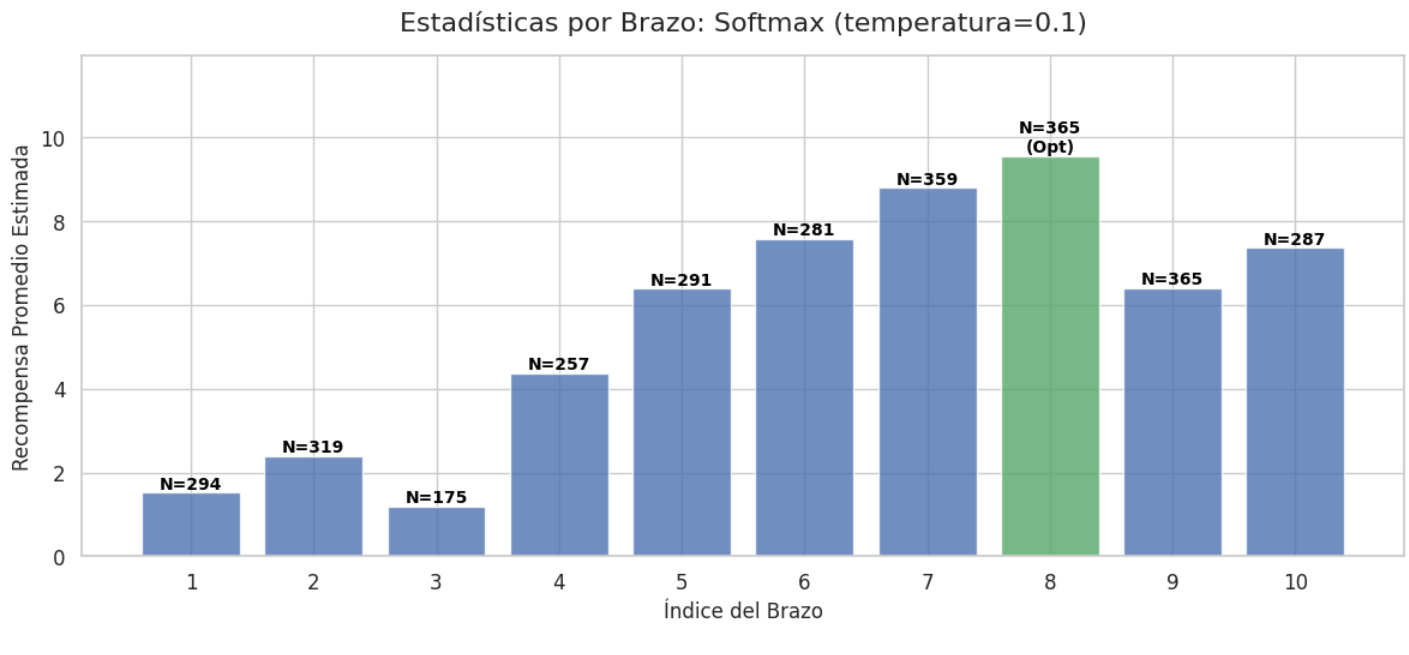
\includegraphics[width=0.5\textwidth]{resources/softmax_histograma.png}
\caption{Histograma de selección de brazos con distribución Normal para el algoritmo Softmax con temperatura $tau = 0.1$.}
\label{fig:softmax_histograma1}
\end{figure}

\begin{figure}
\centering
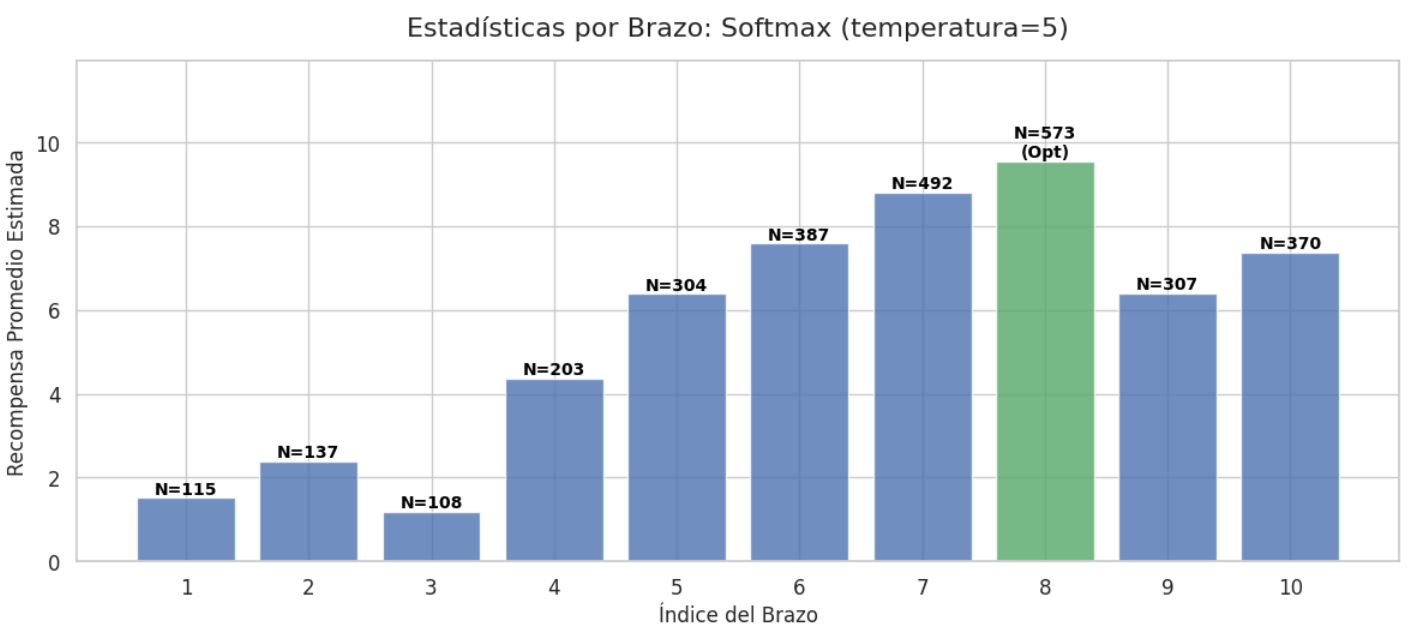
\includegraphics[width=0.5\textwidth]{resources/softmax_histograma2.png}
\caption{Histograma de selección de brazos con distribución Normal para el algoritmo Softmax con temperatura $tau = 5.0$.}
\label{fig:softmax_histograma2}
\end{figure}

Además, se observó que el regret acumulado crece de manera lineal para todas las distribuciones, a diferencia de 
los algoritmos de la familia UCB que presentan un crecimiento logarítmico. Esto lo podemos ver por ejemplo para la 
distribución Normal en la Figura \ref{fig:softmax_regret}, pero es un comportamiento que se repite para las otras distribuciones.

\begin{figure}
\centering
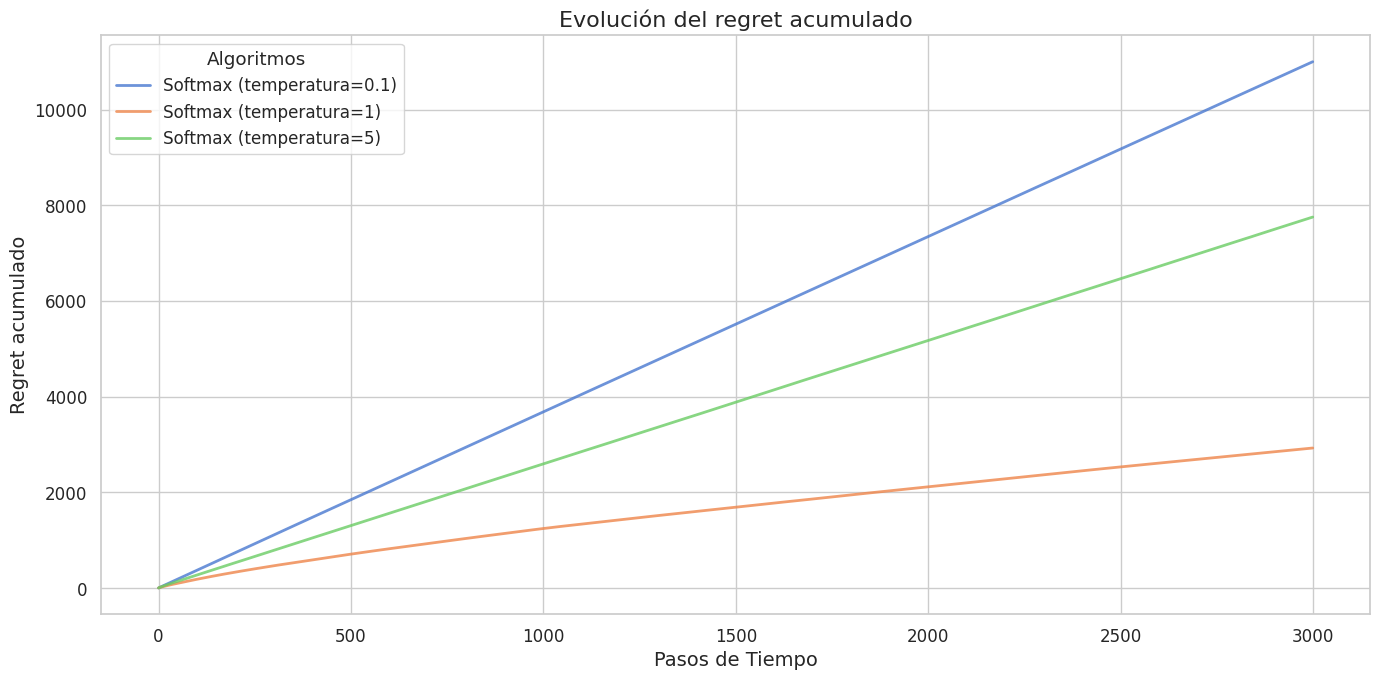
\includegraphics[width=0.5\textwidth]{resources/softmax_regret.png}
\caption{Evolución del regret acumulado para el algoritmo Softmax con distribución Normal.}
\label{fig:softmax_regret}
\end{figure}

\paragraph{Resultados distintos en la distribución de Bernoulli}
Al analizar los resultados en la distribución de Bernoulli , se detectó una anomalía 
positiva en el rendimiento de la temperatura baja ($\tau=0.1$). A diferencia del caso Normal, 
donde $\tau=0.1$ fallaba estrepitosamente, en el entorno binario su rendimiento mejoró notablemente, 
acercándose al de $\tau=5.0$.

Este fenómeno se atribuye a la naturaleza discreta y penalizadora de la distribución 
Bernoulli (recompensas de 0 o 10).
\begin{enumerate}
    \item Cuando el algoritmo voraz ($\tau=0.1$) selecciona un brazo subóptimo y recibe una recompensa de 0 
    (fracaso), el promedio estimado de dicho brazo cae drásticamente.
    \item Debido a la baja temperatura, esta caída en el valor $Q$ reduce la probabilidad de selección del 
    brazo a casi cero de forma inmediata.
    \item Los ``ceros'' actúan como un mecanismo de seguridad que fuerza al algoritmo a abandonar los óptimos 
    locales y seguir explorando, mitigando el riesgo de estancamiento típico de las políticas voraces.
\end{enumerate}

Esto se puede ver en la gráfica de la Figura \ref{fig:softmax_bernoulli} donde se observa que la 
recompensa promedio obtenida con $\tau=0.1$ es muy similar a la obtenida con $\tau=5.0$:
\begin{figure}
\centering
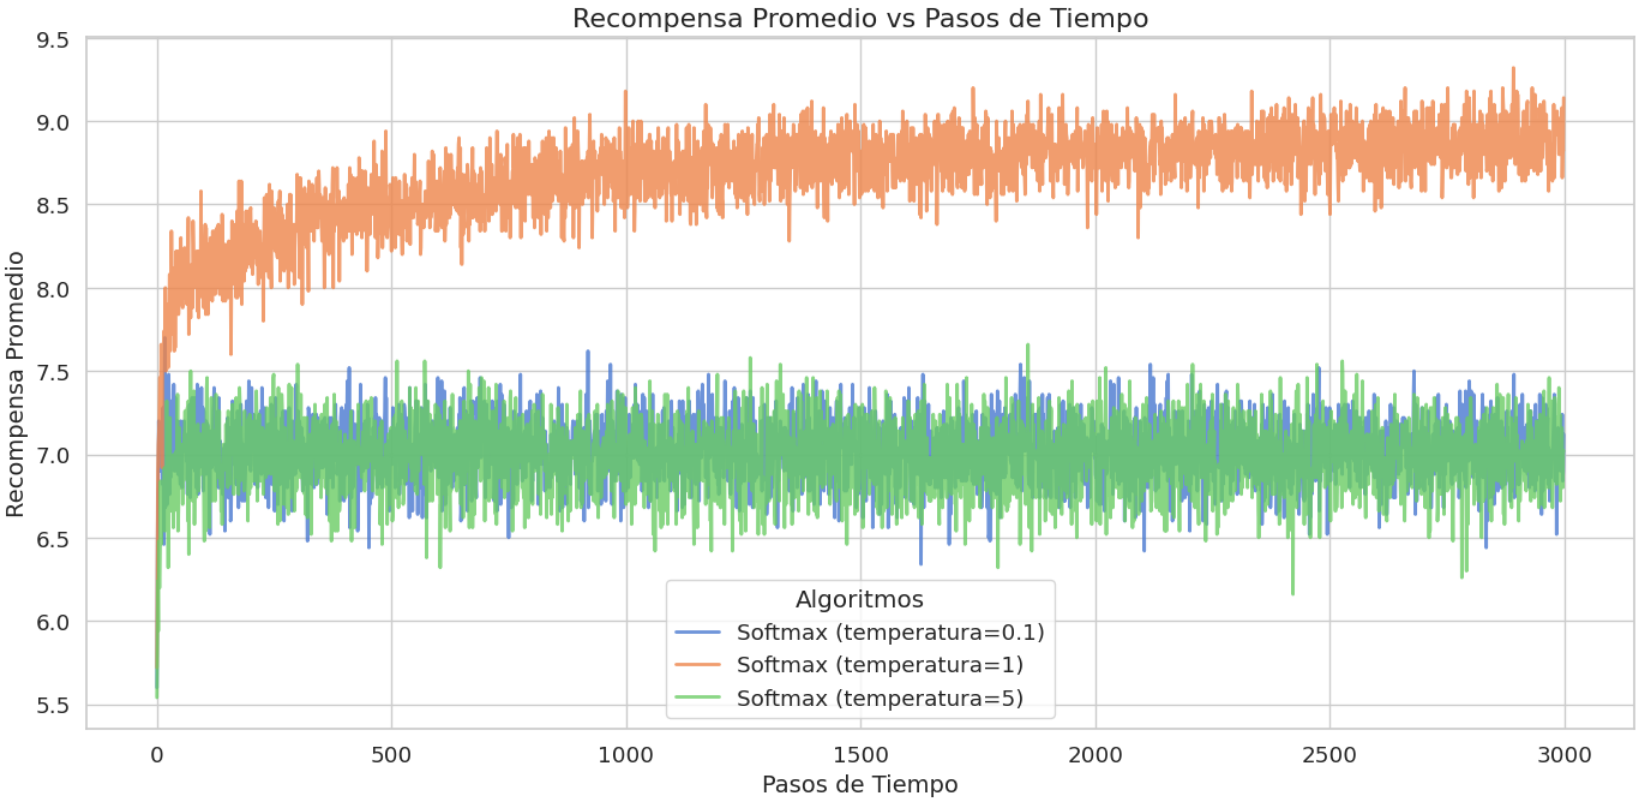
\includegraphics[width=0.5\textwidth]{resources/softmax_bernoulli.png}
\caption{Evolución de la recompensa promedio para el algoritmo Softmax con distribución de Bernoulli.}
\label{fig:softmax_bernoulli}
\end{figure}

\subsubsection{Experimento Adicional: Impacto de la Exploración Inicial}

Dado que la configuración de baja temperatura ($\tau = 0.1$) tiende a converger prematuramente a 
óptimos locales debido a su comportamiento voraz, se diseñó un experimento adicional para 
mitigar este defecto. Se introdujo una fase de \textbf{exploración inicial forzada}, obligando
al agente a seleccionar cada uno de los $k$ brazos una vez antes de aplicar la política Softmax estándar, al igual
que se realiza en el algoritmo $epsilon$-greedy. Estos resultados se encuentran en la Figura \ref{fig:softmax_exploracion_inicial}.

\begin{figure}
\centering
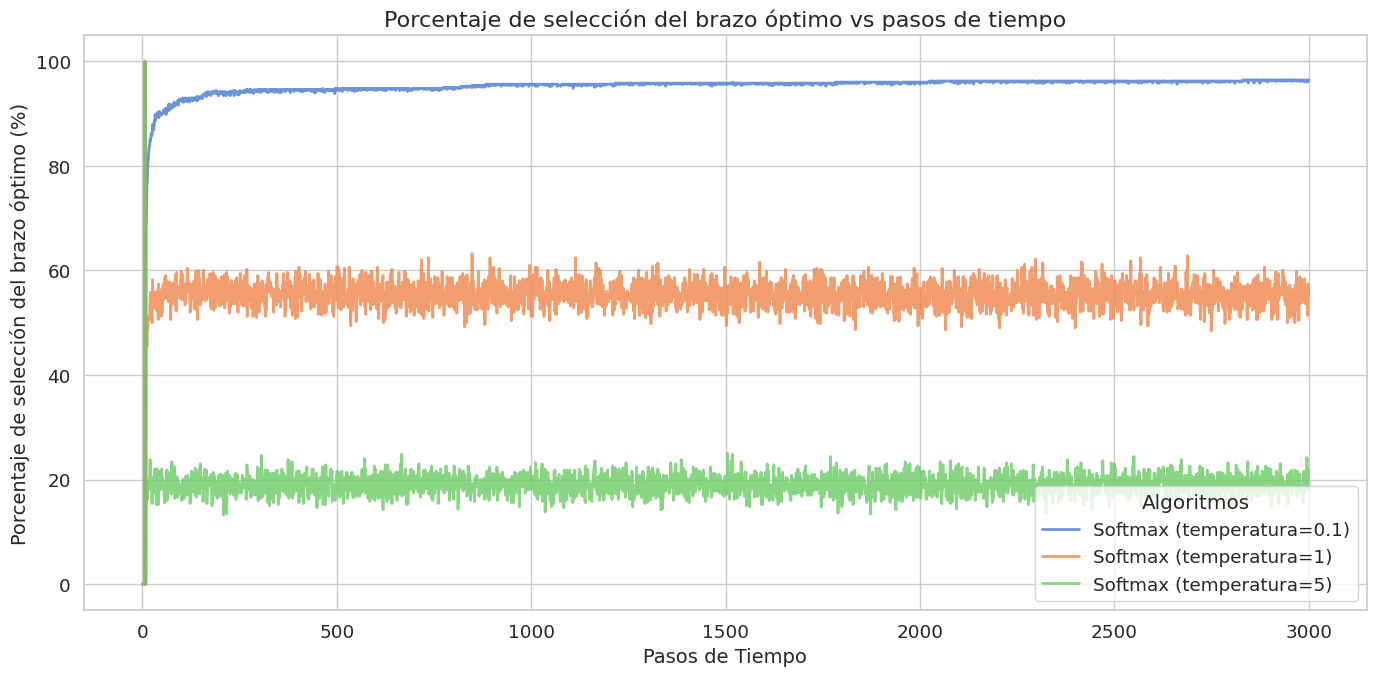
\includegraphics[width=0.5\textwidth]{resources/softmax_exploracion_inicial.png}
\caption{Evolución del porcentaje de selección del brazo óptimo para el algoritmo Softmax con distribución Normal con fase de exploración inicial forzada.}
\label{fig:softmax_exploracion_inicial}
\end{figure}

\textbf{Resultados obtenidos:}
\begin{itemize}
    \item \textbf{Mejora Crítica en $\tau=0.1$:} Esta primera pasada transformó radicalmente el rendimiento de esta configuración. Al garantizar una estimación inicial de todas las medias, el agente pudo identificar y explotar el brazo óptimo casi inmediatamente.
    \item \textbf{Aceleración de la Convergencia:} Se observó una reducción drástica en el tiempo de estabilización del algoritmo, pasando de aproximadamente 3000 pasos (en la versión estándar) a converger cerca de los 500 pasos.
    \item \textbf{Impacto Marginal en $\tau \ge 1.0$:} Para temperaturas medias y altas, la exploración inicial no aportó mejoras significativas, dado que la propia entropía de la distribución de Gibbs con estos valores ya garantiza una exploración suficiente por sí misma.
\end{itemize}

Este experimento confirma que las políticas casi-voraces ($\tau \to 0$) son viables y altamente eficientes si se combinan
con una fase de exploración inicial que garantice una cobertura mínima de todas las acciones.

\subsection{Resultados: Familia UCB (Upper Confidence Bound)}

Se evaluaron los algoritmos UCB1 y UCB2, en el caso de UCB1 variando el parámetro de exploración $C \in \{0.5, 1, 2\}$ y en el de UCB2 variando la duración de épocas $\alpha \in \{0.1, 0.01, 0.001\}$.

Para todas las distribuciones, se observó que:
\begin{itemize}
    \item \textbf{UCB1:} El agente presenta siempre un buen aprovechamiento de la información previamente adquirida, 
    con una curva de aprendizaje muy pronunciada. La variación de $C$ modifica de manera suave el equilibrio entre 
    exploración y explotación. Con $C=2.0$, el agente se comporta de manera más exploradora, mientras que con $C=0.5$
    se vuelve más voraz, como se puede observar en la Figura \ref{fig:ucb_histograma1}.
    \item \textbf{UCB2}: También es un algoritmo muy eficaz, alcanzando en rendimientos similares y en algunos casos 
    superiores a UCB1. Al trabajar con épocas, los agentes presentan un comportamiento oscilatorio entre explotación 
    del brazo óptimo y exploración de brazos subóptimos, que depende del parámetro $\alpha$. El valor $\alpha=0.1$ 
    mostró el mejor rendimiento en nuestros experimentos, seguido usualmente por $\alpha=0.001$. Sin embargo, para el 
    valor intermedio de $\alpha=0.01$ las oscilaciones mencionadas tenían un periodo de orden de magnitud similar al 
    horizonte temporal del experimento, lo que causaba una caída considerable en el rendimiento en la mitad de cada 
    ejecución, como se puede observar en la Figura \ref{fig:ucb_histograma2}. 
\end{itemize}
\begin{figure}
\centering
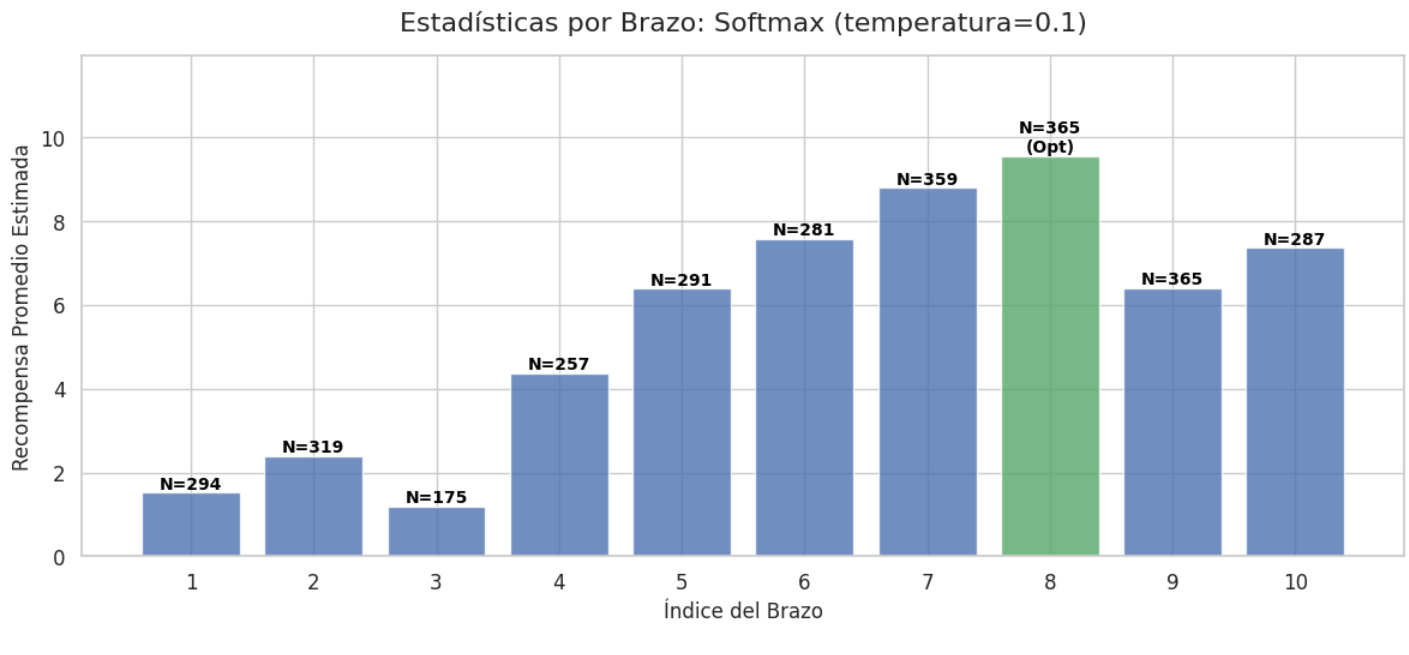
\includegraphics[width=0.5\textwidth]{resources/softmax_histograma.png}
\caption{Histograma de selección de brazos con distribución Normal para el algoritmo Softmax con temperatura $tau = 0.1$.}
\label{fig:softmax_histograma1}
\end{figure}

\begin{figure}
\centering
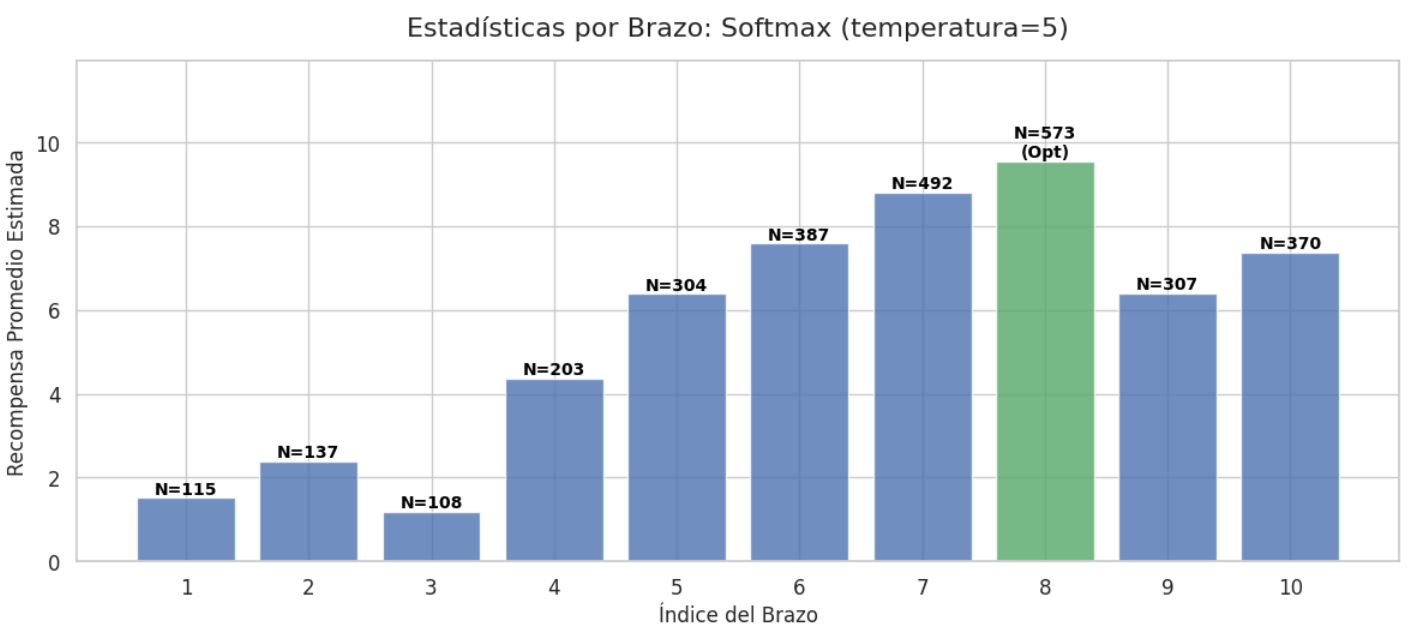
\includegraphics[width=0.5\textwidth]{resources/softmax_histograma2.png}
\caption{Histograma de selección de brazos con distribución Normal para el algoritmo Softmax con temperatura $tau = 5.0$.}
\label{fig:softmax_histograma2}
\end{figure}

Además, se observó que el regret acumulado crece de manera lineal para todas las distribuciones, a diferencia de 
los algoritmos de la familia UCB que presentan un crecimiento logarítmico. Esto lo podemos ver por ejemplo para la 
distribución Normal en la Figura \ref{fig:softmax_regret}, pero es un comportamiento que se repite para las otras distribuciones.

\begin{figure}
\centering
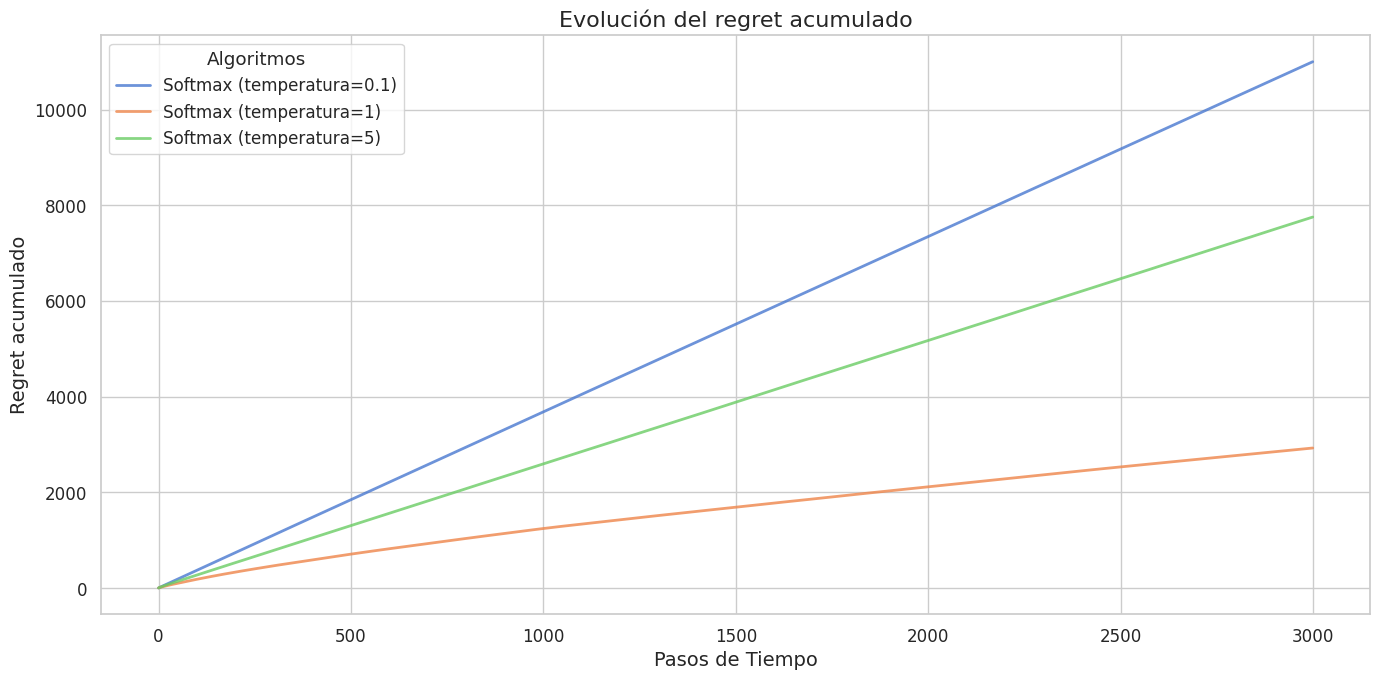
\includegraphics[width=0.5\textwidth]{resources/softmax_regret.png}
\caption{Evolución del regret acumulado para el algoritmo Softmax con distribución Normal.}
\label{fig:softmax_regret}
\end{figure}

\paragraph{Resultados distintos en la distribución de Bernoulli}
Al analizar los resultados en la distribución de Bernoulli , se detectó una anomalía 
positiva en el rendimiento de la temperatura baja ($\tau=0.1$). A diferencia del caso Normal, 
donde $\tau=0.1$ fallaba estrepitosamente, en el entorno binario su rendimiento mejoró notablemente, 
acercándose al de $\tau=5.0$.

Este fenómeno se atribuye a la naturaleza discreta y penalizadora de la distribución 
Bernoulli (recompensas de 0 o 10).
\begin{enumerate}
    \item Cuando el algoritmo voraz ($\tau=0.1$) selecciona un brazo subóptimo y recibe una recompensa de 0 
    (fracaso), el promedio estimado de dicho brazo cae drásticamente.
    \item Debido a la baja temperatura, esta caída en el valor $Q$ reduce la probabilidad de selección del 
    brazo a casi cero de forma inmediata.
    \item Los ``ceros'' actúan como un mecanismo de seguridad que fuerza al algoritmo a abandonar los óptimos 
    locales y seguir explorando, mitigando el riesgo de estancamiento típico de las políticas voraces.
\end{enumerate}

Esto se puede ver en la gráfica de la Figura \ref{fig:softmax_bernoulli} donde se observa que la 
recompensa promedio obtenida con $\tau=0.1$ es muy similar a la obtenida con $\tau=5.0$:
\begin{figure}
\centering
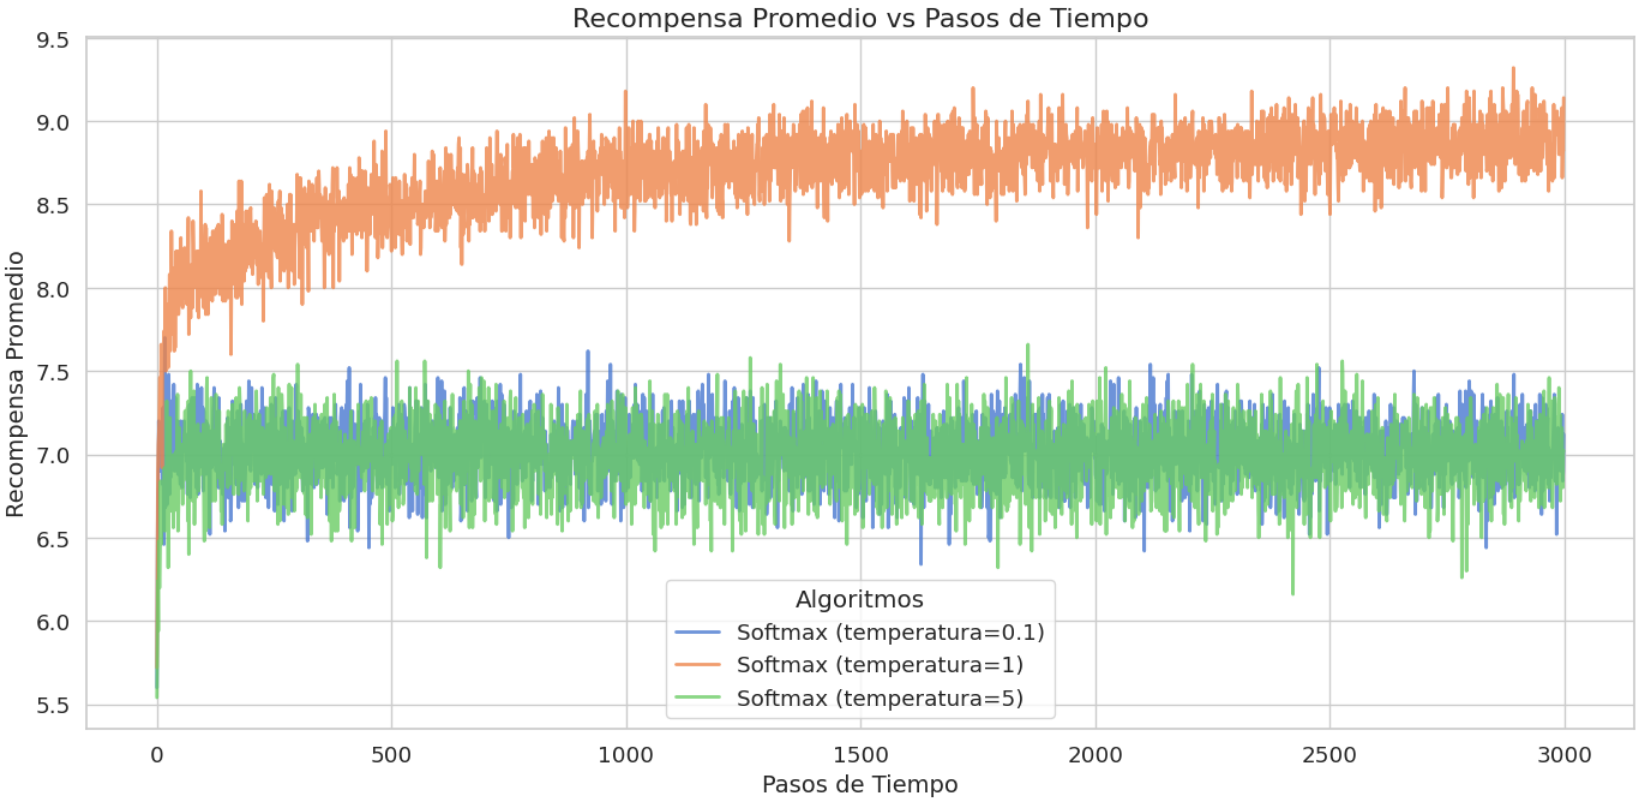
\includegraphics[width=0.5\textwidth]{resources/softmax_bernoulli.png}
\caption{Evolución de la recompensa promedio para el algoritmo Softmax con distribución de Bernoulli.}
\label{fig:softmax_bernoulli}
\end{figure}

\subsubsection{Experimento Adicional: Impacto de la Exploración Inicial}

Dado que la configuración de baja temperatura ($\tau = 0.1$) tiende a converger prematuramente a 
óptimos locales debido a su comportamiento voraz, se diseñó un experimento adicional para 
mitigar este defecto. Se introdujo una fase de \textbf{exploración inicial forzada}, obligando
al agente a seleccionar cada uno de los $k$ brazos una vez antes de aplicar la política Softmax estándar, al igual
que se realiza en el algoritmo $epsilon$-greedy. Estos resultados se encuentran en la Figura \ref{fig:softmax_exploracion_inicial}.

\begin{figure}
\centering
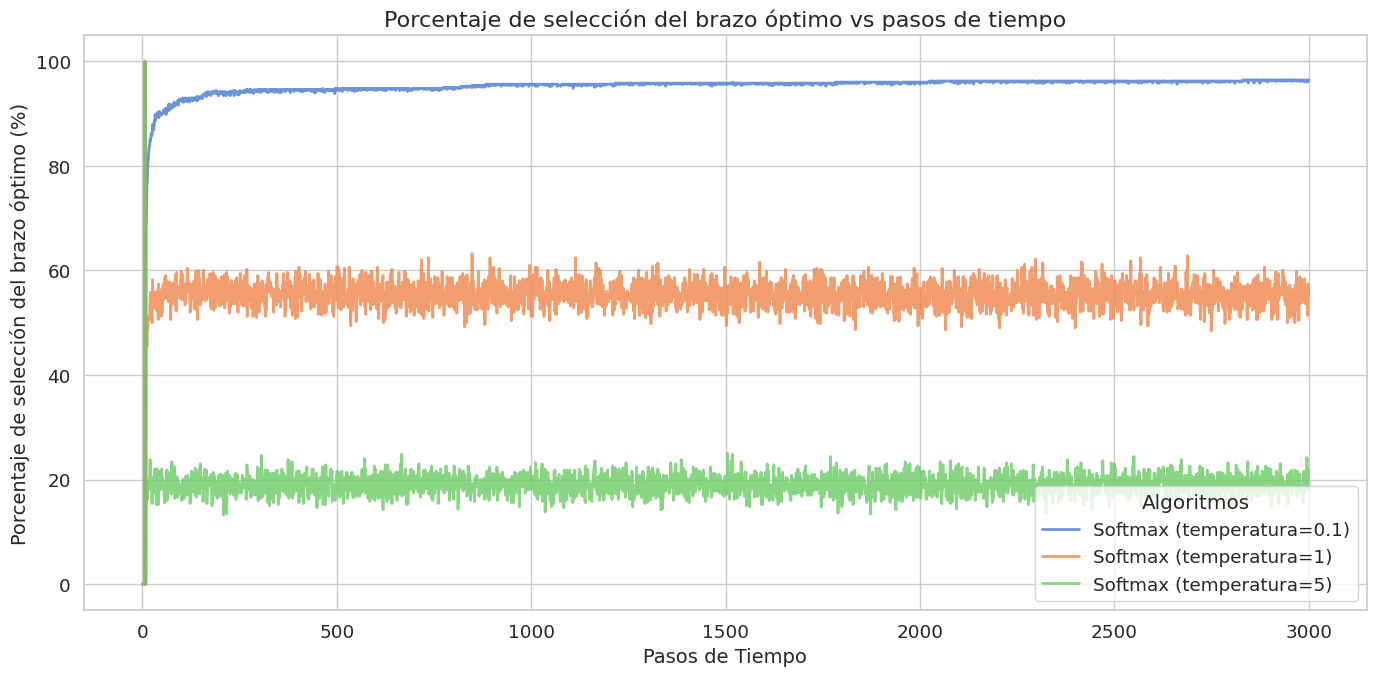
\includegraphics[width=0.5\textwidth]{resources/softmax_exploracion_inicial.png}
\caption{Evolución del porcentaje de selección del brazo óptimo para el algoritmo Softmax con distribución Normal con fase de exploración inicial forzada.}
\label{fig:softmax_exploracion_inicial}
\end{figure}

\textbf{Resultados obtenidos:}
\begin{itemize}
    \item \textbf{Mejora Crítica en $\tau=0.1$:} Esta primera pasada transformó radicalmente el rendimiento de esta configuración. Al garantizar una estimación inicial de todas las medias, el agente pudo identificar y explotar el brazo óptimo casi inmediatamente.
    \item \textbf{Aceleración de la Convergencia:} Se observó una reducción drástica en el tiempo de estabilización del algoritmo, pasando de aproximadamente 3000 pasos (en la versión estándar) a converger cerca de los 500 pasos.
    \item \textbf{Impacto Marginal en $\tau \ge 1.0$:} Para temperaturas medias y altas, la exploración inicial no aportó mejoras significativas, dado que la propia entropía de la distribución de Gibbs con estos valores ya garantiza una exploración suficiente por sí misma.
\end{itemize}

Este experimento confirma que las políticas casi-voraces ($\tau \to 0$) son viables y altamente eficientes si se combinan
con una fase de exploración inicial que garantice una cobertura mínima de todas las acciones.


\subsection{Análisis Comparativo Global}

Se realizó un experimento conjunto utilizando una distribución Normal con $\mu \in [1,10]$, $\sigma=1$, $k=10$ brazos, 500 ejecuciones y 1000 pasos, comparando cinco algoritmos: $\epsilon$-Greedy ($\epsilon=0.01$), $\epsilon$-decaimiento ($\epsilon_0=1$, $\lambda=0.01$, $\epsilon_{min}=0.01$), UCB1 ($c=1$), UCB2 ($\alpha=0.1$) y Softmax ($\tau=0.1$).

\subsubsection{Discusión de Resultados}

\begin{itemize}
    \item \textbf{Convergencia y selección óptima:} UCB2 mostró el mejor comportamiento global, alcanzando aproximadamente un 99\% de selección del brazo óptimo, seguido muy de cerca por UCB1 (98\%). Ambos métodos presentan una convergencia rápida y estable gracias a su exploración dirigida basada en incertidumbre. Softmax (95\%) y $\epsilon=0.01$ (89\%) mantienen una exploración residual constante, lo que limita su convergencia al 100\%. A $\epsilon$-decaimiento (91\%) le ocurre lo mismo, y además, su elevada exploración inicial disminuye su recompensa promedio al principio.

    La comparación directa del porcentaje de selección óptima se presenta en la Figura~\ref{fig:global_optimal_selection}.

    \begin{figure}[H]
    \centering
    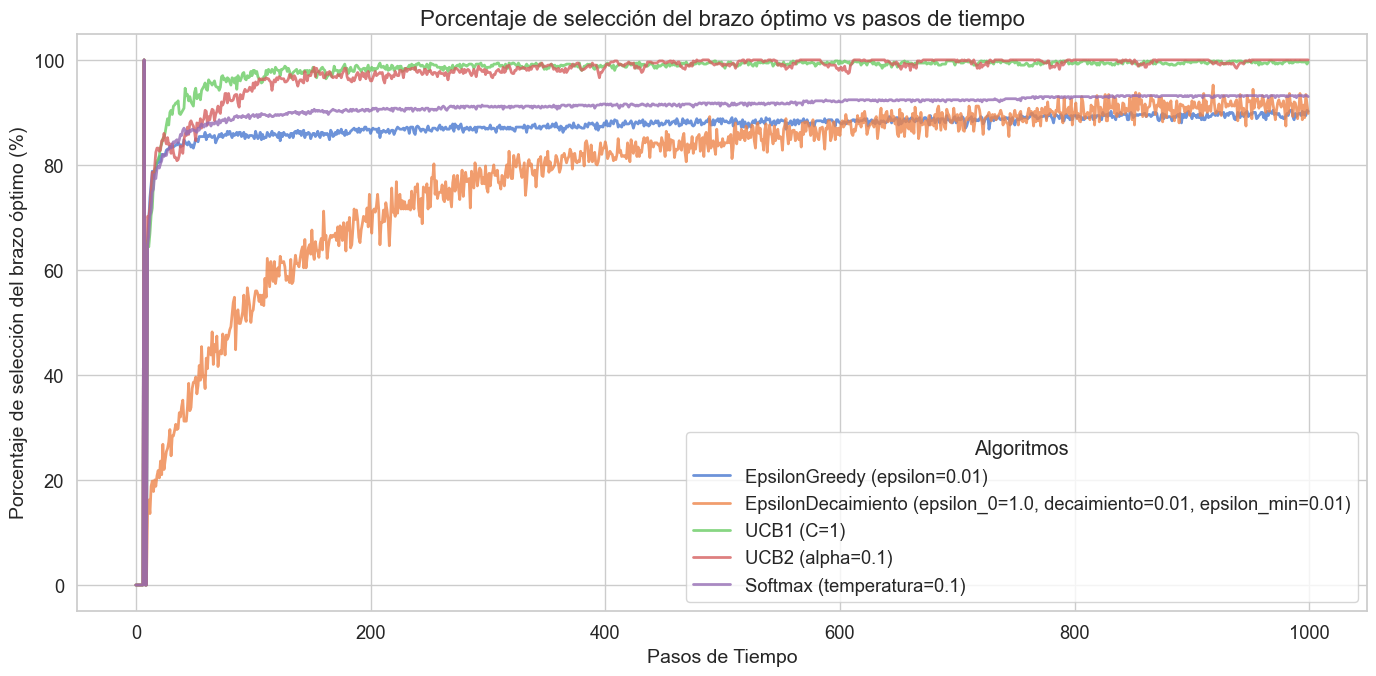
\includegraphics[width=0.5\textwidth]{resources/global_optimal_selection.png}
    \caption{Porcentaje de selección del brazo óptimo en el experimento comparativo global.}
    \label{fig:global_optimal_selection}
    \end{figure}


    \item \textbf{Rendimiento en recompensa promedio:} Salvo $\epsilon$-decaimiento, todos los algoritmos convergen rápidamente hacia la media del brazo óptimo (9.56 en esta instancia). UCB1, UCB2, Softmax y $\epsilon=0.01$ alcanzan prácticamente el mismo valor final. El $\epsilon$-decaimiento presenta un crecimiento más lento debido al coste inicial de exploración, aunque con un horizonte mayor tendería al mismo nivel.

    La evolución de la recompensa promedio puede observarse en la Figura~\ref{fig:global_reward}.

    \begin{figure}[H]
    \centering
    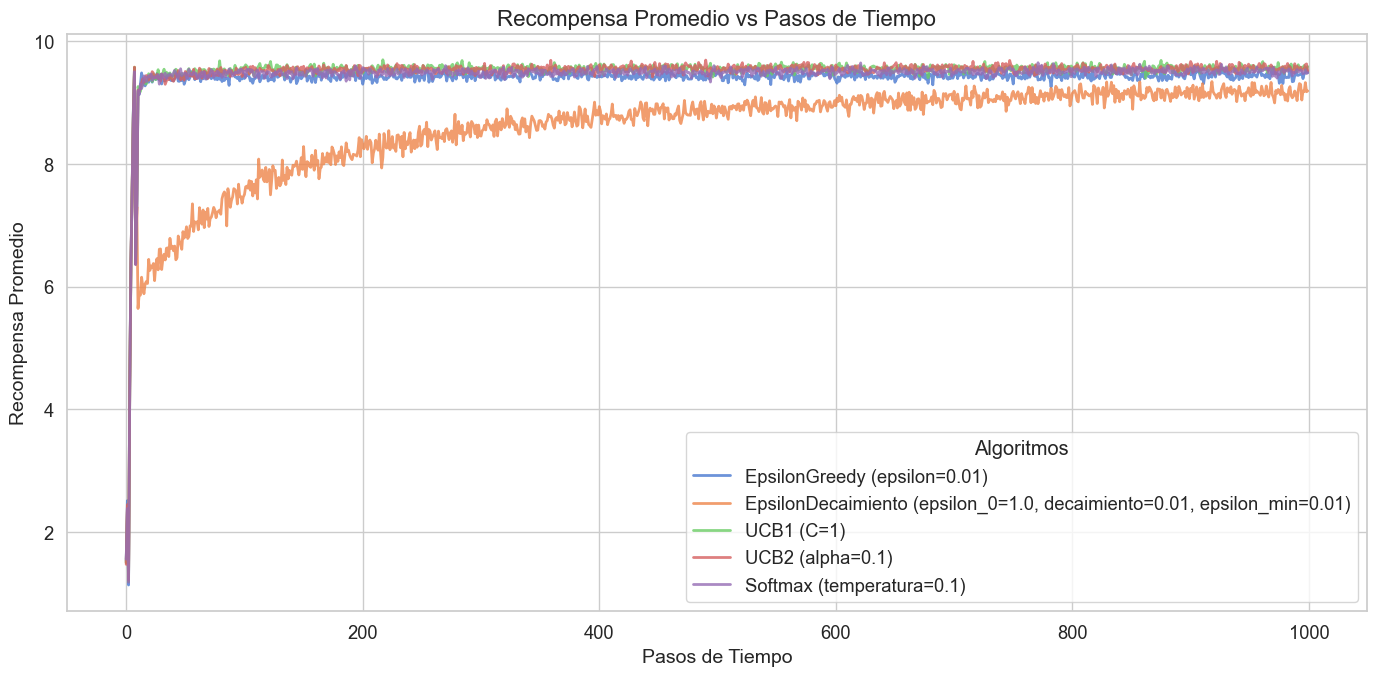
\includegraphics[width=0.5\textwidth]{resources/global_reward_comparison.png}
    \caption{Recompensa promedio acumulada en el experimento comparativo global.}
    \label{fig:global_reward}
    \end{figure}


    \item \textbf{Regret acumulado:} UCB1 y UCB2 mantienen el menor regret global. Softmax y $\epsilon=0.01$ presentan un crecimiento moderado debido a su exploración constante. $\epsilon$-decaimiento acumula mayor regret en las primeras fases, lo que afecta su rendimiento observable en horizontes finitos.

    El comportamiento del regret acumulado se muestra en la Figura~\ref{fig:global_regret}.

    \begin{figure}[H]
    \centering
    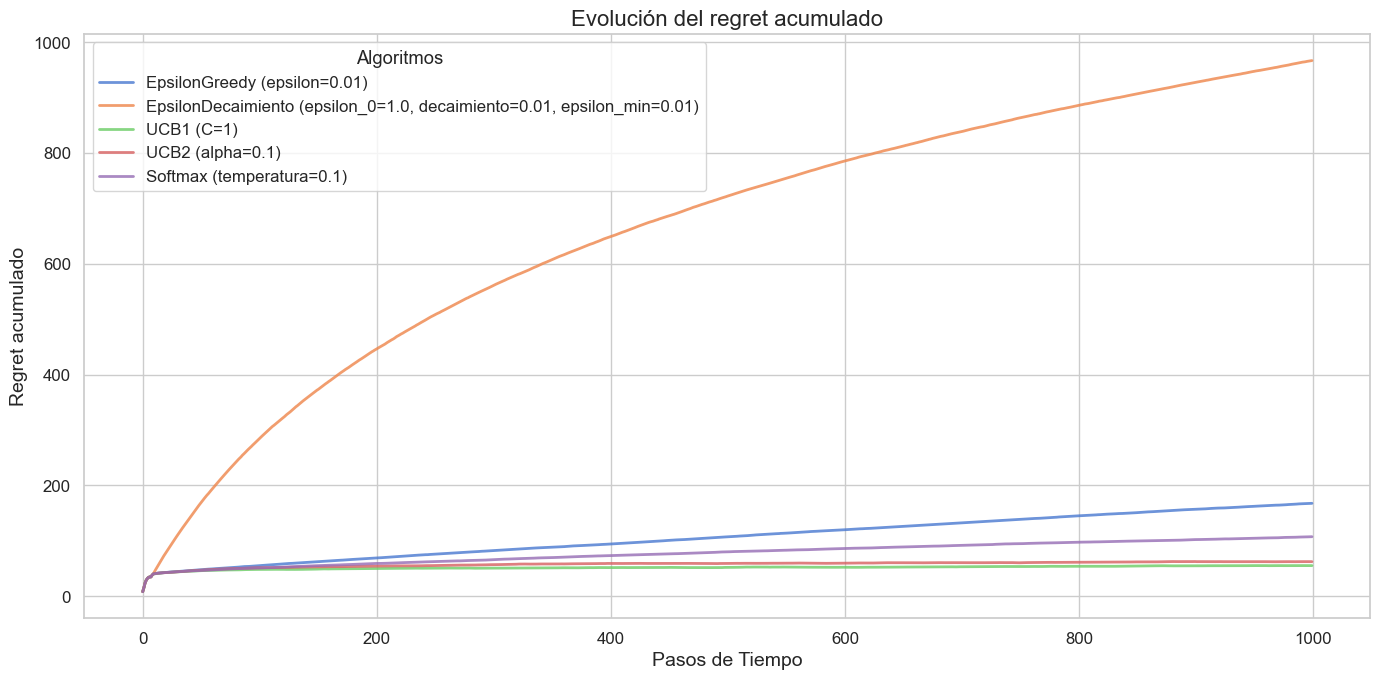
\includegraphics[width=0.5\textwidth]{resources/global_regret_comparison.png}
    \caption{Regret acumulado en el experimento comparativo global.}
    \label{fig:global_regret}
    \end{figure}


    \item \textbf{Conclusión:} En este experimento concreto, UCB2 se posiciona como la estrategia más eficiente y robusta, combinando rápida convergencia, máxima selección óptima y bajo regret. UCB1 ofrece resultados prácticamente equivalentes. Softmax y $\epsilon$-Greedy con $\epsilon$ pequeño son competitivos en recompensa promedio, pero estructuralmente menos eficientes en términos de identificación de brazon óptimo. El esquema con decaimiento resulta más sensible al horizonte temporal considerado.
\end{itemize}


    

Es posible que para sus resultados use figuras y tablas como la Figura \ref{fig:1} o la Tabla \ref{tab:1}.
Si la tabla fuera demasiado grande use \texttt{sidewaystable} y póngala al final del documento.

\begin{figure}[htb!]
\centering
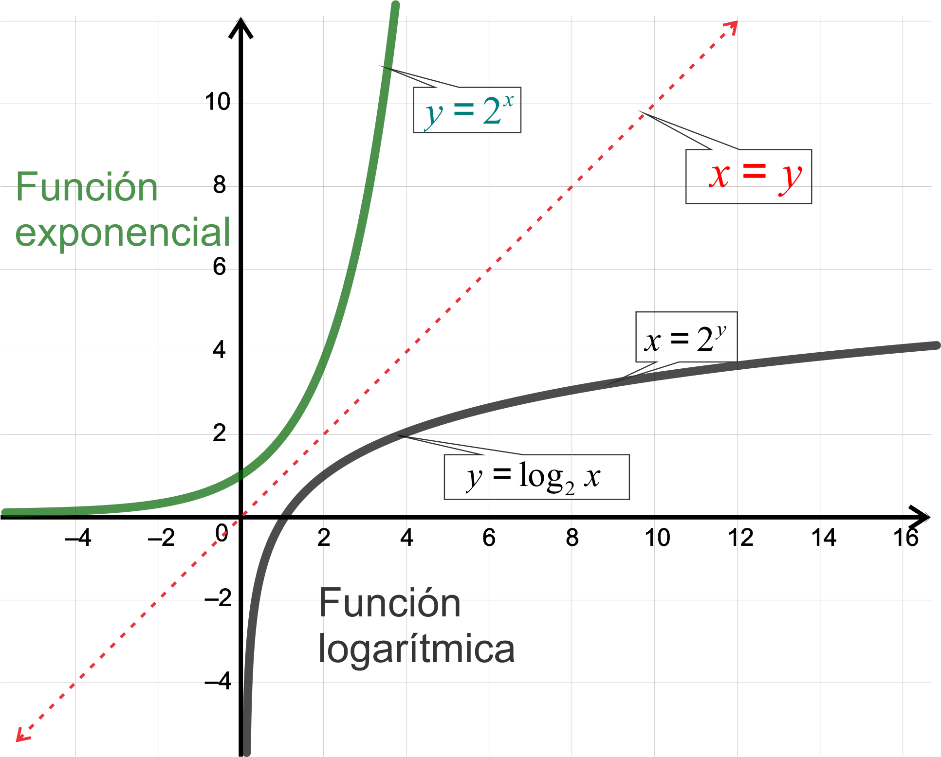
\includegraphics[width=0.45\textwidth]{exponencial}
\caption{Esto es un ejemplo de figura}\label{fig:1}
\end{figure}






\begin{table}[htb!]
\caption{Ejemplo de Tabla}\label{tab:1}%
\centering
\begin{tabular}{@{}llll@{}}
\toprule
Column 1 & Column 2  & Column 3 & Column 4\\
\midrule
row 1    & data 1   & data 2  & data 3  \\
row 2    & data 4   & data 5\footnotemark[1]  & data 6  \\
row 3    & data 7   & data 8  & data 9\footnotemark[2]  \\
\bottomrule
\end{tabular}
\begin{itemize}
    \item[$^1$] tablefootnote 1
    \item[$^2$] tablefootnote 2
  \end{itemize}
\end{table}
% Deben estar fuera del entorno flotante. % Si se quieren las marcas al pie de página
%\footnotetext[1]{Ejemplo de footnote para una celda de tabla}
%\footnotetext[2]{Ejemplo de footnote para una celda de tabla}



%%%%%%%%%%%%%%%%%%%%%%%%%%%%%%%%%%%%%%%%%%%%%%%%%%%%%%%%%%%%%
%%%%%%%%%%%%%%%%%%%%%%%%%%%%%%%%%%%%%%%%%%%%%%%%%%%%%%%%%%%%%   
\section{Conclusiones}
    \begin{itemize}
        \item Un resumen de los principales resultados obtenidos.
        \item Limitaciones del estudio y posibles mejoras futuras.
        \item Reflexión sobre la importancia del trabajo y su impacto en el campo del aprendizaje por refuerzo.
        \item Líneas \textit{futuras} de estudio.
    \end{itemize}

